%%%%%%%%%%%%%%%%%%%%%%%%%%%%%%%%%%%%%%%%%%%%%%%%%%%%%%%%
%                       Assignment 2                   %
%                                                      %
% Author: Michael P. J. Camilleri					   %
%                                                      %
% Based on the Cleese Assignment Template for Students %
% from http://www.LaTeXTemplates.com.				   %
%                                                      %
% Original Author: Vel (vel@LaTeXTemplates.com)		   %
%													   %
% License:											   %
% CC BY-NC-SA 3.0 									   %
% (http://creativecommons.org/licenses/by-nc-sa/3.0/)  %
% 													   %
%%%%%%%%%%%%%%%%%%%%%%%%%%%%%%%%%%%%%%%%%%%%%%%%%%%%%%%%

%--------------------------------------------------------
%   IMPORTANT: Do not touch anything in this part
\documentclass[12pt]{article}
%%%%%%%%%%%%%%%%%%%%%%%%%%%%%%%%%%%%%%%%%
% Cleese Assignment
% Structure Specification File
% Version 1.0 (27/5/2018)
%
% This template originates from:
% http://www.LaTeXTemplates.com
%
% Author:
% Vel (vel@LaTeXTemplates.com)
%
% License:
% CC BY-NC-SA 3.0 (http://creativecommons.org/licenses/by-nc-sa/3.0/)
% 
%%%%%%%%%%%%%%%%%%%%%%%%%%%%%%%%%%%%%%%%%

%----------------------------------------------------------------------------------------
%	PACKAGES AND OTHER DOCUMENT CONFIGURATIONS
%----------------------------------------------------------------------------------------

\usepackage{lastpage} % Required to determine the last page number for the footer
\usepackage{graphicx} % Required to insert images
\setlength\parindent{0pt} % Removes all indentation from paragraphs
\usepackage[most]{tcolorbox} % Required for boxes that split across pages
\usepackage{booktabs} % Required for better horizontal rules in tables
\usepackage{listings} % Required for insertion of code
\usepackage{etoolbox} % Required for if statements
\usepackage{geometry} % Required for adjusting page dimensions and margins
\usepackage[utf8]{inputenc} % Required for inputting international characters
\usepackage[T1]{fontenc} % Output font encoding for international characters
\usepackage{fancyhdr} % Required for customising headers and footers
\usepackage{xspace}
\usepackage{booktabs}
\usepackage[colorlinks]{hyperref}
\usepackage{etoolbox}

\newcommand{\ie}{i.e.\@\xspace}
\newcommand{\eg}{e.g.\@\xspace}
\newcommand{\notemark}[1]{\textcolor{blue}{N.B.\ \emph{#1}}}
\newcommand{\noteself}[1]{\textcolor{red}{Thought: \emph{#1}}}
\newcommand{\note}[1]{\emph{\textbf{N.B.}\@\xspace#1}}
\newcommand{\hint}[1]{\emph{Hint: #1}}
\newcommand{\half}{$\frac{1}{2}$ }

\newbool{clearnext}		%Running Counter to see if clearing the page or not in the next subquestion.
\newbool{clearon}		%Parameter for specifying whether we will be clearing or not.
\newbool{authoron}		%Parameter to specify whether to show author or not

%----------------------------------------------------------------------------------------
%	Standard Template
%----------------------------------------------------------------------------------------
\geometry{
	paper=a4paper, % Change to letterpaper for US letter
	top=3cm, % Top margin
	bottom=3cm, % Bottom margin
	left=2.5cm, % Left margin
	right=2.5cm, % Right margin
	headheight=14pt, % Header height
	footskip=1.4cm, % Space from the bottom margin to the baseline of the footer
	headsep=1.2cm, % Space from the top margin to the baseline of the header
	%showframe, % Uncomment to show how the type block is set on the page
}
\pagestyle{fancy} % Enable custom headers and footers

%----------------------------------------------------------------------------------------
%	My Changes
%----------------------------------------------------------------------------------------
\lhead{\small\assignmentClass}
\chead{}
\ifbool{authoron}{\rhead{\small{\assignmentAuthorName}}}{\rhead{}}

\lfoot{} % Left footer
\cfoot{} % Centre footer
\rfoot{\small Page\ \thepage\ of\ \pageref{LastPage}} % Right footer

\renewcommand\headrulewidth{0.5pt} % Thickness of the header rule

%----------------------------------------------------------------------------------------
%	MODIFY SECTION STYLES
%----------------------------------------------------------------------------------------

\usepackage{titlesec} % Required for modifying sections

%------------------------------------------------
% Section

\titleformat
{\section} % Section type being modified
[block] % Shape type, can be: hang, block, display, runin, leftmargin, rightmargin, drop, wrap, frame
{\Large\bfseries} % Format of the whole section
{\assignmentQuestionName~\thesection} % Format of the section label
{6pt} % Space between the title and label
{} % Code before the label

\titlespacing{\section}{0pt}{0.5\baselineskip}{0.5\baselineskip} % Spacing around section titles, the order is: left, before and after

%------------------------------------------------
% Subsection

\titleformat
{\subsection} % Section type being modified
[block] % Shape type, can be: hang, block, display, runin, leftmargin, rightmargin, drop, wrap, frame
{} % Format of the whole section
{[\arabic{section}.\arabic{subsection}]} % Format of the section label (\alph{subsection})
{4pt} % Space between the title and label
{} % Code before the label

\titlespacing{\subsection}{0pt}{0.5\baselineskip}{0.5\baselineskip} % Spacing around section titles, the order is: left, before and after

\renewcommand\thesubsection{(\alph{subsection})}

%----------------------------------------------------------------------------------------
%	CUSTOM QUESTION COMMANDS/ENVIRONMENTS
%----------------------------------------------------------------------------------------

% Environment to be used for each question in the assignment
\newenvironment{question}[1]{
	\ifbool{clearon}{\clearpage}{}
	\global\setbool{clearnext}{false}
	\vspace{0.5\baselineskip} % Whitespace before the question
	\section{: #1}
	\lfoot{\small\itshape\assignmentQuestionName~\thesection~continued on next page\ldots} % Set the left footer to state the question continues on the next page, this is reset to nothing if it doesn't (below)
}{
	\lfoot{} % Reset the left footer to nothing if the current question does not continue on the next page
}

%------------------------------------------------

% Environment for inter-subquestion texts (no arguments)
\newenvironment{interquestiontext}{
	\ifbool{clearon}{\ifbool{clearnext}{\clearpage}{}}{}
	\global\setbool{clearnext}{false}
}{
}

%------------------------------------------------


%------------------------------------------------

% Environment for subquestions, takes 1 argument - the name of the section
\newenvironment{subquestion}[1]{
	\ifbool{clearon}{\ifbool{clearnext}{\clearpage}{}}{}
	\global\setbool{clearnext}{true}
	\subsection{#1}
}{
}

%------------------------------------------------

% Command to print a question sentence
\newcommand{\questiontext}[1]{
	\textbf{#1}
	\vspace{0.5\baselineskip} % Whitespace afterwards
	\global\setbool{clearnext}{false}
}

%------------------------------------------------
% Command to print a  Marking Scheme box.
\newcommand{\marking}[1]{
	\begin{tcolorbox}[colback=green!5!white,enhanced]
		\textbf{Marking Scheme:}#1
	\end{tcolorbox}
}

%------------------------------------------------

% Command to print a box that breaks across pages with the space for a student to answer
\newcommand{\model}[1]{
	\begin{tcolorbox}[enhanced]
		\textbf{Model Answer}:#1
	\end{tcolorbox}
}

\newcommand{\answerbox}[2]{
	\begin{tcolorbox}[enhanced, height=#1]
		#2
	\end{tcolorbox}
}

%------------------------------------------------

% Command to print an assignment section title to split an assignment into major parts
\newcommand{\assignmentSection}[1]{
	{
		\centering % Centre the section title
		\vspace{2\baselineskip} % Whitespace before the entire section title
		
		\rule{0.8\textwidth}{0.5pt} % Horizontal rule
		
		\vspace{0.75\baselineskip} % Whitespace before the section title
		{\LARGE \MakeUppercase{#1}} % Section title, forced to be uppercase
		
		\rule{0.8\textwidth}{0.5pt} % Horizontal rule
		
		\vspace{\baselineskip} % Whitespace after the entire section title
	}
}

%----------------------------------------------------------------------------------------
%	TITLE PAGE
%----------------------------------------------------------------------------------------

\title{
	\thispagestyle{empty} 		% Suppress headers and footers
	\vspace{0.01\textheight} 	% Whitespace before the title
	\textbf{\assignmentClass:\\ \assignmentTitle}\\[4pt]
	\ifbool{authoron}{\assignmentAuthorName}{
	\ifdef{\assignmentDueDate}{{\small Due\ on\ \assignmentDueDate}\\}{}
	{\large \textit{\assignmentWarning}}
	\vspace{0.01\textheight}} % Whitespace before the author name
}

\ifbool{authoron}{\author{Student: \textbf{\assignmentAuthorName}}}{}
\date{} % Don't use the default title page date field





% Options for Formatting Output

\global\setbool{clearon}{true} %
\global\setbool{authoron}{true} %



\newcommand{\assignmentQuestionName}{Question}
\newcommand{\assignmentTitle}{Assignment\ \#2}

\newcommand{\assignmentClass}{IAML -- INFR11182 (LEVEL 11)}

\newcommand{\assignmentWarning}{NO LATE SUBMISSIONS} % 
\newcommand{\assignmentDueDate}{Friday,\ November\ 15,\ 2019 @ 16:00}
%--------------------------------------------------------

%--------------------------------------------------------
%   IMPORTANT: Specify your Student ID below [You will need to uncomment the line, else compilation will fail]. Make sure to specify your student ID correctly, otherwise we may not be able to identify your work and you will be marked as missing.
\newcommand{\assignmentAuthorName}{s1980787}
%--------------------------------------------------------

\begin{document}
\maketitle
\thispagestyle{empty}



%%%%%%%%%%%%%%%%%%%%%%%%%%%%%%%%%%%%%%%%%%%%%%%%%%%%%%%%%%%%%%%%%%%%%%%%%%%%%%
%============================================================================%
%%%%%%%%%%%%%%%%%%%%%%%%%%%%%%%%%%%%%%%%%%%%%%%%%%%%%%%%%%%%%%%%%%%%%%%%%%%%%%


\assignmentSection{Part A: 20-NewsGroups [77 Points]}




\begin{question}{(10 points) Exploratory Analysis}

\questiontext{We will begin by exploring the Dataset to get some insight about it.}



\begin{subquestion}{(5 points) Focusing first on the training set, summarise the key features/observations in the data: focus on the dimensionality, data ranges, feature and class distribution and report anything out of the ordinary. What are the typical values of the features like?}


\answerbox{12em}{
As we expected, the dimensionality of the training dataset is extremely high (1000 columns) plus the target class. We expected that since we have a total of 1000 words used in the newsgroups, and each word is a feature itself. The most frequent value for a feature is 0 (sparse dataset), which is normal because we know that in a comment/text very few words will be present. We have 5648 documents. The value that each attribute takes is in the range [0,1]. Using a histogram to visualize the class distribution of the training data, we see that all the classes except "talk.religion.misc" contain almost the same number of documents (around 750, but class7 only around 460).
}



\end{subquestion}


\begin{subquestion}{(3 points) Looking now at the Testing set, how does it compare with the Training Set (in terms of sizes and feature-distributions) and what could be the repurcussions of this?}


\answerbox{10em}{
The proportion of training/test set is good (75-25), and we observe the same class distribution. However, in training set we have smaller mean in the features, but the mean maximum value is almost 1. In contrast, in testing set we have a bigger mean but the mean maximum value is 0.86. That means that the documents contain a wider distribution of words, but do not contain "strong" words in order to make it more clear for which one is its class. 
}



\end{subquestion}

\begin{subquestion}{(2 points) Why do you think it is useful to consider TF-IDF weights as opposed to just the frequency of times a word appears in a document as a feature?}



\answerbox{10em}{
TF-IDF is way more useful than using just frequency of times a word appears in a document. TF-IDF actually is giving a metric of how much "important" a word is in the particular document since it is takes into account if the word occurs in other documents too. If so, then the value will be smaller which means that it gives us less information about the correlation between the document and the class. 
}



\end{subquestion}



\end{question}


%============================================================================%

\begin{question}{\label{Q_UNSUP_LEARN}(24 points) Unsupervised Learning}

\questiontext{We will now explore the documents in some detail by way of clustering.}



\begin{subquestion}{(2 points) The K-Means algorithm is non-deterministic. Explain why this is, and how the final model is selected in the SKLearn implementation of \href{https://scikit-learn.org/stable/modules/clustering.html}{KMeans}.}



\answerbox{8em}{
The k-means algorithm is not deterministic since its initialization includes a random selection of the centroids. This means that running the algorithm several times on the same data, could give different results. The implementation on SKLearn does not select randomly the position of the centroids, but initializes them to be generally distant from each other, leading to provably better results than random initialization.
}



\end{subquestion}


\begin{subquestion}{(1 point) One of the parameters we need to specify when using k-means is the number of clusters. What is a reasonable number for this problem and why?}



\answerbox{5em}{
The number of class labels gives us the number of K. Since we have 8 different labels on the data, we can say that K = 8.
}



\end{subquestion}


\begin{subquestion}{(5 points) We will use the Adjusted Mutual Information (AMI) \ie \href{https://scikit-learn.org/stable/modules/clustering.html\#mutual-info-score}{\texttt{adjusted\_mutual\\\_info\_score}} between the clusters and the true (known) labels to quantify the performance of the clustering. Give an expression for the MI in terms of entropy. In short, describe what the MI measures about two variables, why this is applicable here and why it might be difficult to use in practice. \hint{MI is sometimes referred to as Information Gain: note that you are asked only about the standard way we defined MI and not the AMI which is adjusted for the size of the domain and for chance agreement.}}



\answerbox{16em}{
An expression about the information gain in terms of entropy can be given with the following expression.
\[ MI(X;Y) = H(Y) - H(Y|X) \]
This expression, in other words says that, the information gain is equal to the amount of uncertainty of Y which is removed by knowing X.

This is applicable here, since we know the class of each instance X. This does not happen when clustering is used, because it is unsupervised and we do not know the target. That is why it is very difficult to have information gain about two variables in practice.
}



\end{subquestion}

\begin{subquestion}{(4 points) Fit K-Means objects with \texttt{n\_clusters} ranging from 2 to 12. Set the random seed to 1000 and the number of initialisations to 50, but leave all other values at default. For each fit compute the adjusted mutual information (there is an SKLearn \href{https://scikit-learn.org/stable/modules/generated/sklearn.metrics.adjusted_mutual_info_score.html}{function} for that). Set \texttt{average\_method=`max'}. Plot the AMI scores against the number of clusters (as a line plot).}



\answerbox{40em}{
\begin{center}
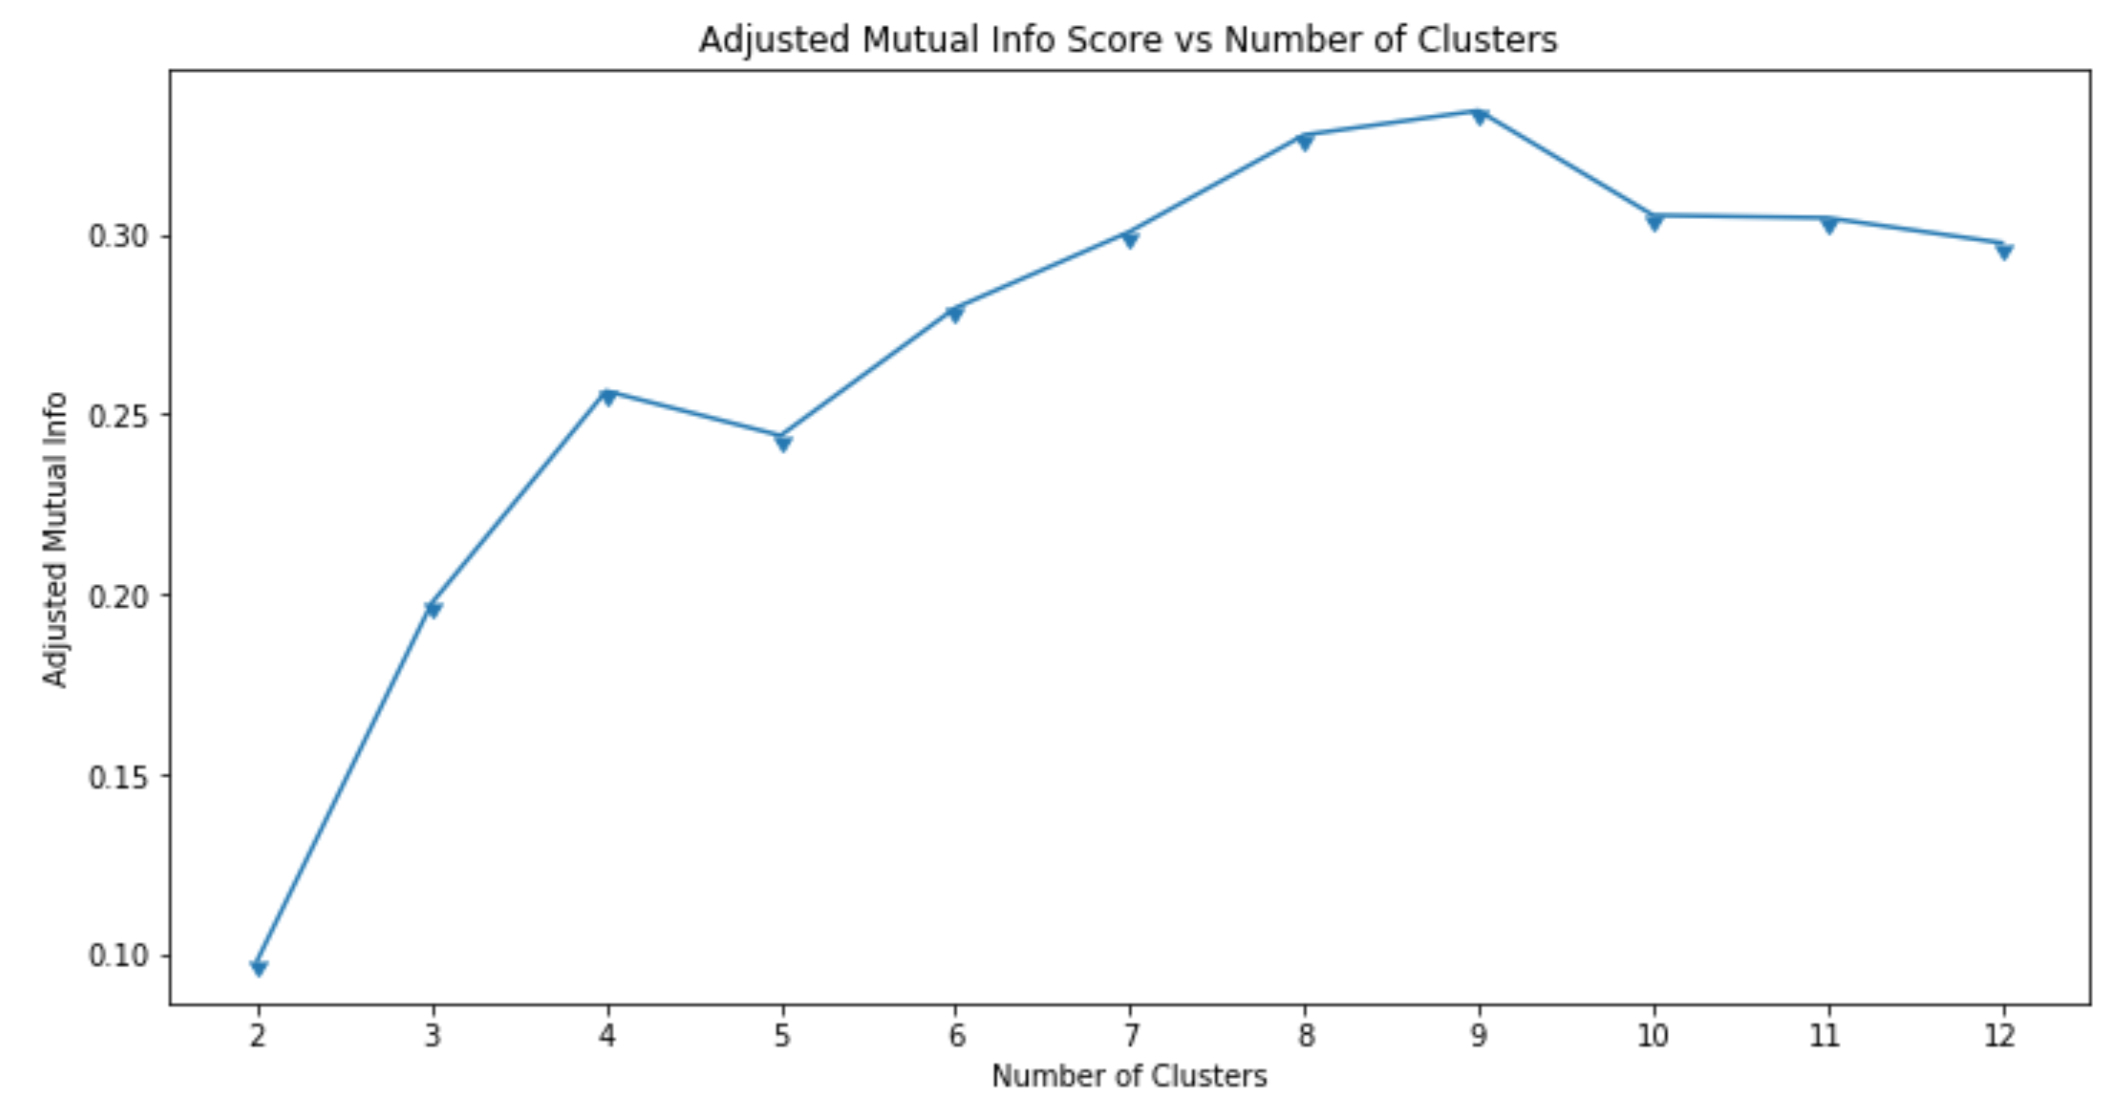
\includegraphics[scale=0.57]{../Plots/AMI.png}
\end{center}
}



\end{subquestion}

\begin{subquestion}{(3 points) Discuss any trends and interesting aspects which emerge from the plot. Does this follow from your expectations?}



\answerbox{10em}{
We can say that the plot has the shape we expected. We see the trend that for a small number of clusters, the AMI we gain is low, and while the number of clusters gets bigger, AMI increases too. However, that does not hold for K = 4 and K = 5. After a particular number of clusters, the information gain, starts to decrease (big number of clusters does not mean a better model). An interesting observation is that the optimal number of clusters it is not K = 8 (8 class targets in data) but K=9. However, there is only a small difference between the AMI these two gain.
}



\end{subquestion}

\begin{subquestion}{\label{Q_CLUSTER_FOUR}(6 points) Let us investigate the case with four (4) clusters in some more detail. Using seaborn's \href{https://seaborn.pydata.org/generated/seaborn.countplot.html}{\texttt{countplot}} function, plot a bar-chart of the number of data-points with a particular class (encoded by colour) assigned to each cluster centre (encoded by position on the plot's x-axis). As part of the cluster labels, include the total number of data-points assigned to that cluster.}



\answerbox{40em}{
\begin{center}
\includegraphics[scale=0.55]{../Plots/cluster_labels_k4.png}
\end{center}
}



\end{subquestion}

\begin{subquestion}{(3 points) How does the clustering in Question\ref{Q_UNSUP_LEARN}:\ref{Q_CLUSTER_FOUR} align with the true class labels? Does it conform to your observations in Q 2(e)?}



\answerbox{14em}{
From the plot in the question 2.6 we see that the cluster 3 contains over the half of the instances. It seems that in clusters 0, 1 and 2, the classification is clear, since we observe some consistency on the data classification. However, this is not observed in the cluster 3, which has a large number of instances from all classes classified to it. In cluster 3, it is very difficult to observe a pattern, and we can say that this messes the clustering. That's why we have a low AMI for k = 4, as we have seen in Q2.5. Although, the three clusters give information about the data, with cluster 3 is very difficult to export conclusions and that leads the information gain not to be larger. 
}



\end{subquestion}



\end{question}

%============================================================================%

\begin{question}{(26 points) Logistic Regression Classification}
\label{Q_LR_NG}
\questiontext{We will now try out supervised classification on this data. We will focus on Logistic Regression and measure performance in terms of the \href{https://scikit-learn.org/stable/modules/generated/sklearn.metrics.f1_score.html}{F1} score (familiarise yourself with this score which is related to the precision and recall scores that we learnt about in class).}



\begin{subquestion}{(3 points) What is the F1-score, and why is it preferable to accuracy in our problem? How does the macro-average work to extend the score to multi-class classification?}



\answerbox{8em}{
F1-score is a useful metric of evaluation which is used to combine two other very useful metrics into a single number (Precision and Recall). It is always between these two numbers. It is preferable to accuracy, since we have an uneven class distribution and therefore accuracy would be a bad metric. A macro-average computes the metric independently for each class and then takes the average (treating all classes equally).
}



\end{subquestion}


\begin{subquestion}{(2 points) As always we start with a simple baseline classifier. Define such a classifier (indicating why you chose it) and report its performance on the \textbf{Test} set. Use the `macro' average for the \texttt{f1\_score}.} %\hint{For the baseline, the classifier should use only the target labels.}



\answerbox{8em}{
As we can see from the data distribution, the most frequent class is class 6. However this happens with a very small difference from other classes. That's why it is preferable not using a baseline predicting the most frequent class, but use a random classifier. Since it is random, we take the average f1score after 100 iterations which is 0.13. 
}



\end{subquestion}

\begin{subquestion}{(3 points) We will now train a \href{https://scikit-learn.org/stable/modules/generated/sklearn.linear_model.LogisticRegression.html}{LogisticRegression} Classifier from SKLearn. By referring to the documentation, explain how the Logistic Regression model can be applied to classify multi-class labels as in our case. \hint{Limit your explanation to methods we discussed in the lectures.}}



\answerbox{9em}{
Logistic Regression is a binary classifier, which means that it can classify an instance if it is in one class or not. For multiclass, the method classifies the data into k and not-k. This method is found in the documentation with the name "OvR - One vs Rest". In OvR Logistic Regression a seperate model is trained for each class predicting whether an instance is in that class or not, using the softmax function and assigning the instance to the class with the greatest probability.
}



\end{subquestion}

\begin{subquestion}{(4 points) Train a Logistic Regressor on the training data. Set \texttt{solver=`lbfgs'}, \texttt{multi\_class=`multinomial'} and \texttt{random\_state=0}. Use the Cross-Validation object you created and report the average validation-set F1-score as well as the standard deviation. Comment on the result.}



\answerbox{9em}{
Validation set f1score = 0.669, Validation set Standard Deviation = 0.017\\
As we can see, the model here is way more accurate in terms of f1score comparing it to the baseline we used. The standard deviation of the f1score on the validation set is almost zero, so the validation set is well distributed, since there are no differences on the f1score in each fold.
}



\end{subquestion}

\begin{subquestion}{\label{Q_LOG_REG_PLT}(5 points) We will now optimise the Regularisation parameter $C$ using cross-validation. Train a logistic regressor for different values of $C$: in each case, evaluate the F1 score on the training and validation portion of the fold. That is, for each value of $C$ you must provide the training set and validation-set scores per fold and then compute (and store) the average of both over all folds. Finally plot the (average) training and validation-set scores as a function of $C$. \hint{Use a logarithmic scale for $C$, spanning 19 samples between $10^{-4}$ to $10^5$.}}



\answerbox{40em}{
\includegraphics[scale=0.55]{../Plots/RegularisationC_with_geomspace.png}
}



\end{subquestion}

\begin{subquestion}{(7 points) What is the optimal value of $C$ (and the corresponding score)? How did you choose this value? By making reference to the effect of the regularisation parameter $C$ on the optimisation, explain what is happening in your plot from Question \ref{Q_LR_NG}:\ref{Q_LOG_REG_PLT} \hint{Refer to the documentation for $C$ in the \href{https://scikit-learn.org/stable/modules/generated/sklearn.linear_model.LogisticRegression.html}{LogisticRegression} page on SKLearn}.}



\answerbox{11em}{
We see from the plot, that for small values of C, the performance is very low. But while we increase the value of parameter C, the performance gets better, until we reach the maxium performance. Small values of C increase the regularization which means that simpler models are created, underfitting the data. By using bigger values of C, the model increases its complexity and adjust better to the data. However, if we increase the value of C too much, it overfits the data. I selected C=1 (f1score = 0.669), since it seems that although it is not the optimal value for training set, this is the optimal value of C in validation set. 
}



\end{subquestion}

\begin{subquestion}{(2 points) Finally, report the score of the best model on the test-set, after retraining on the entire training set (that is drop the folds). \hint{You may need to set \texttt{max\_iter = 200}.} Comment briefly on the result.}



\answerbox{7em}{
After retraining on the entire training set and using C=1, the score for the test set is 0.6748. This is very close to the f1 score we got from the validation set, using the regularisation paramenter C=1. 
}



\end{subquestion}


\end{question}




%============================================================================%



\begin{question}{(17 points) Hierarchical Classification}

\questiontext{We will now leverage the structure of the target labels to try out hierarchical classification.}



\begin{subquestion}{(2 Marks) What aspects of the data may lend to better classification in such a hierarchical fashion?
}



\answerbox{10em}{
The data now are classified into 4 superclasses which are more clearly separated than before. The problem we faced in k-means when the number of clusters was 4, now it no longer exists. The data are seperated in the 4 superclasses which are like 4 different datasets, and the classification can be done to each of the superclass seperately, in order to find the class of each instance.
}



\end{subquestion}

\begin{subquestion}{(3 points) First train a Logistic Regressor on the high-level classes (\ie the four super-labels): use the same setup as before (Question \ref{Q_LR_NG}), optimising the regularisation parameter $C$ over the folds. Report the best validation-set F1-score (average over folds) together with the optimal value of $C$. \hint{Remember to keep track of the \textbf{best} classifier trained on the \textbf{entire} dataset (\ie training data with no folds).}} Can we compare this result to the previous ones?



\answerbox{8em}{
The best validation set f1score is 0.8266 when the value of parameter C = 0.316. The score is high, since we predicted the superclasses. The boundaries between the superclasses are more clear. We cannot compare this result with the previous ones, since they are completely different things. Previously we had to classify the data into 8 classes, but now only 4.
}



\end{subquestion}

\begin{subquestion}{(2 points) We will now train individual binary classifiers for each of the groups. Why should we use the true super-class targets and not the ones predicted from the above classifier?}



\answerbox{8em}{
Since we have a classification problem, the target values are known, so we use these in order to evaluate the model. The superclasses which were predicted from the above classifier, contain some misclassifications, which will lead to false results. So we use the known superclass labels, to evaluate the model. Using the true labels, we assume that we have 4 different datasets, completely unrelated with each other, so the results will be better.
}



\end{subquestion}

\begin{subquestion}{(7 points) Train four independent Logistic Regression (binary) classifiers on the two classes within each super-group. That is, for each super-group, extract only the samples corresponding to that super-group using the true group label, then optimise a Logistic Regression classifier on the data with the targets being the two classes in that super-group. Report in each case the regularisation value which gives the best validation-set score as well as the associated F1-score. \hint{This would look best in a table. Also, remember to keep track of the best classifier trained on the entire group in each case.}}



\answerbox{9em}{
\includegraphics[scale=0.22]{../Plots/hierarchical_4groups_cgeo.png}
}



\end{subquestion}

\begin{subquestion}{(3 points) Using the trained classifiers in a hierarchical fashion, evaluate the resulting model on the testing set for the full 8-way classification. \hint{You will need to first generate the group-level predictions using the base classifier, and then, conditioned on this, predict the individual labels. Make sure to construct the indices correctly}. How does this compare to the original single-layer classifier?}



\answerbox{6em}{
It seems that the hierarchical classification works much worse (f1score = 0.25) on the dataset than the single layer classifier. This happens because we have a bad classification when we try to assign the superclasses to the instances and then since we have some error there, the error will be enlarged in binary classifications.
}



\end{subquestion}

\end{question}




%%%%%%%%%%%%%%%%%%%%%%%%%%%%%%%%%%%%%%%%%%%%%%%%%%%%%%%%%%%%%%%%%%%%%%%%%%%%%%
%============================================================================%
%%%%%%%%%%%%%%%%%%%%%%%%%%%%%%%%%%%%%%%%%%%%%%%%%%%%%%%%%%%%%%%%%%%%%%%%%%%%%%

\clearpage

\assignmentSection{Part B: Bristol Air-Quality [98 points]}




\begin{question}{\label{Q_EXPLORATORY}(30 Points) Exploratory Analysis}

\questiontext{We will begin by exploring the Dataset to familiarise ourselves with it.}



\begin{subquestion}{(6 points) Summarise the key features/observations in the data: describe the purpose of each column and report (briefly) also on the dimensionality/ranges (ballpark figures only, and how they compare across features) and number of sites, and identify anything out of the ordinary/problematic: \ie look out for missing data and negative values. Why are the latter unreasonable in such a dataset? \hint{Refer to the documentation for how to interpret the pollutant values.}}



\answerbox{13em}{
We see that the dataset consist of a very big number of instances, but a small number of attributes. This is good, since we have a large dataset, so we will get more reliable results. The dimensionality of the dataset is low, however, some attributes can be removed and the information will not be lost, since they are not independent. Clearly, these attributes are Loc.Lat and Loc.Long, which can be removed, since the information the give can be extracted from the SiteID (18 different places). In addition, the three columns NOx, NO2 and NO, can have some dependence to each other, so one or two of them can be removed, without losing much information. We can also observe a large number of null and negative values, fact that it is unreasonable since the observation values should be above 0.
}



\end{subquestion}

\begin{subquestion}{(6 points) Repeat the same analysis but this time on a per-site basis. Provide a table with the number of samples and percentage of problematic samples (negative and missing) in each site. To report numbers, count a row which has at least one missing entry
as having missing data, and similarly for negative entries. \hint{Pandas has a handy method, \texttt{to\_latex()}, for generating a latex table from a dataframe.}}



\answerbox{17em}{
\includegraphics[scale=0.6]{../Plots/t1_new.png}
\includegraphics[scale=0.6]{../Plots/t2_new.png}

}



\end{subquestion}

\begin{subquestion}{(4 points) Briefly summarise how the sites compare in terms of number of samples and amount of problematic samples.}



\answerbox{11em}{
The number of samples in each site varies from a very small number (site 15) and a very large one (site 1). We are sure that something's not going good with site 15 (all problematic). Sites with also too many problematic samples are the site 3 with a proportion over 3/4, and site 13 with over the half of its samples been problematic. Although the percentages of these problematic sites are extremely high, we see that the number of samples is small for each of these sites. This is good, since they are a very small portion of the data.
}



\end{subquestion}

\begin{subquestion}{(3 points) Given that the columns are all oxides of nitrogen and hence we expect them to be related, we will now look at correlations in our data. This will also be useful in determining how well we can predict any one of the readings from the other two. Remove the data from sites 3 and 15 and compute the \textbf{Pearson} correlation coefficient between each of the three pollutant columns on the remaining data. Visualise the coefficients between each pair of columns in a table.}



\answerbox{10em}{
\includegraphics[scale=0.30]{../Plots/NO_corr.png}
}



\end{subquestion}

\begin{subquestion}{(2 points) Comment on the level of correlation between each pair of pollutants.}



\answerbox{7em}{
We observe a very strong correlation between NOx and NO which is near 1 (nearly linear relationship). That means that there is a dependence between these two columns, and thus one of them can be eliminated without losing information. NO2 is also correlated with the other 2 with a weaker but also strong correlation (better with NOx). 
}



\end{subquestion}



\begin{subquestion}{\label{CORRELATIONS}(5 points) For each of the three pollutants, compute the Pearson correlation between sites. \hint{You will need to remove the `Date Time' column and then group by the first level of the columns.} Then plot these as three heatmaps: show the values within the figures. \hint{Use the method \texttt{plot\_matrix()} from \texttt{mpctools.extensions.mplext}.}}



\answerbox{40em}{
\includegraphics[scale=0.28]{../Plots/NOx.png}
\includegraphics[scale=0.28]{../Plots/NO.png}
\includegraphics[scale=0.28]{../Plots/NO2.png}
}



\end{subquestion}

\begin{subquestion}{(4 points) Comment briefly on your observations from Question \ref{Q_EXPLORATORY}:\ref{CORRELATIONS}: start by summarising the results from the NO gas and then comment on whether the same is observed in the other gases or if there is something different.}



\answerbox{12em}{
Observing the NO heatmap we see that the sites 6,7,12 and 14 have the lowest correlation with the other sites. These sites have the minimum correlation coefficient with each other (7-14: 0.31, 6-7: 0.43, 6-12: 0.46). The other sites seem that they are enough correlated, with correlation coefficient aroud 0.7 which indicates strong correlation. The same conclusions we get observing the other two heatmaps, since they have only very few differences between them. That was something we were sure that would happen since from ex5.4 we found almost a linear relationship between NO and NOx, and a strong correlation between NO and NO2 (0.8).}



\end{subquestion}

\end{question}


%============================================================================%

\begin{question}{(19 Points) Principal Component Analysis}

\questiontext{One aspect which we have not yet explored is the temporal nature of the data. That is, we need to keep in mind that the readings have a temporal aspect to them which can provide some interesting insight. We will explore this next.}



\begin{subquestion}{(1 point) Plot the first 5 lines of data (plot each row as a single line-plot).}



\answerbox{40em}{
\includegraphics[scale=0.55]{../Plots/5lines.png}
}



\end{subquestion}



\begin{subquestion}{(5 points) We will focus first on data solely from Site 1. Extract the data from this site, and run PCA with the number of components set to 72 for now. Set the \texttt{random\_state=0}. On a single graph plot: (i) the percentage of the variance explained by each principal component (as a bar-chart), (ii) the cumulative variance (line-plot) explained by the first $n$ components: (\hint{you should use \href{https://matplotlib.org/3.1.1/api/_as_gen/matplotlib.axes.Axes.twinx.html}{\texttt{twinx()}} to make the plot fit}), \textsl{and}, (iii) mark the point at which the number of components collectively explain at least 95\% of the variance (using a vertical line). \hint{Number components starting from 1.}}



\answerbox{40em}{
\includegraphics[scale=0.47]{../Plots/PCA.png}
}



\end{subquestion}

\begin{subquestion}{(2 points) Interpret and summarise the above plot.}



\answerbox{9em}{
Initially we had 72 dimensions. After the PCA, we see that we can reduce the dimensionality to 11. That number means that if we choose the 11 eigenvectors with the most variance (highest eigenvalues, indicated with bar plot), we can have the 95\% of the total variance of the dataset (indicated with red line - cumulative variance). We see from the graph that after the green line, the variance is too low, and hence the cumulative variance becomes almost steady.
}


\end{subquestion}


\begin{subquestion}{(5 points) Generate three figures, one for the mean and one for each of the first 2 principal components: in each, plot the mean/component as three lines, one for each pollutant throught one day cycle. \hint{You will need to reshape the components appropriately.}}



\answerbox{50em}{
\includegraphics[scale=0.47]{../Plots/pca_mean.png}
\includegraphics[scale=0.47]{../Plots/pc1.png}
\includegraphics[scale=0.47]{../Plots/pc2.png}
}



\end{subquestion}

\begin{subquestion}{(6 points) Focusing on the mean and first principal component, are there any significant patterns which emerge throughout the day? \hint{Think about car usage throughout the day.} What is different when interpreting the mean versus the first component? \hint{Do peaks signify the same thing in both cases?} Looking at the principal components only, are there any significant differences between the pollutants? Why could this be happening? \hint{You can refer to one of the limitations of PCA.}}



\answerbox{16em}{
Observing the plots we have for mean and first principal component, we see many similarities. They follow the same pattern for the pollution through the day, since we have in both plots the peaks at around 8am and 18pm. These are the times that most of the cars are in the road, and then the pollution reaches its peak. 
The first principal component corresponds to a line which passes through the multidimensional mean, and minimizes the sum of squares of the distances of the points from the line. So the peaks in the plots do not signify the same thing. 
Looking now at plot of the second principal component, we observe some differences to the first component. At 8am, time that in the 1st PC we had a peak, in 2nd PC we have nadir. That is happening due to the nature of 2nd PC which is that it has to capture the highest variance from what is left from the 1st. Therefore, the linear combination of these 2 will give a better approach to the original data.
}



\end{subquestion}

\end{question}

%============================================================================%


\begin{question}{\label{Q_LR_BA}(49 points) Regression}


\questiontext{Given our understanding of the correlation between signals and sites, we will now attempt to predict the NOx level for Site 17 given the value at the other sites. We will evaluate our models using the Root Mean Squared Error (RMSE) \ie the square root of the \href{https://scikit-learn.org/stable/modules/generated/sklearn.metrics.mean_squared_error.html}{mean\_squared\_error} score by sklearn.}



\begin{subquestion}{(2 points) First things first: since we are dealing with a supervised task, we will need to split our data into a training and testing set. Furthermore, since some of our regressors will involve hyper-parameter tuning, we will also need a validation set. Use the \texttt{multi\_way\_split()} method from \texttt{mpctools.extensions.skext} to split the data into a Training (60\%), Validation (15\%) and Testing (25\%) set: use the \href{https://scikit-learn.org/stable/modules/generated/sklearn.model_selection.ShuffleSplit.html}{ShuffleSplit} object from sklearn for the \texttt{splitter}. Set the random state to 0. \hint{The method gives you the indices of the split for each set, which can then be applied to multiple matrices.} Report the sizes of each dataset.}



\answerbox{4em}{
train set : 8937, validation set : 2234, test set : 3724
}



\end{subquestion}

\begin{subquestion}{(4 points) Let us start with a baseline. By using only the $y$-values, what baseline regressor can you define (indicate what it does)? Implement it and report the RMSE on the training and validation sets. Interpret this relative to the statistics of the data.}



\answerbox{8em}{
We can use as a baseline a predictor which always says that the predicted value is the mean of the target values of the training set. In this exercise the baseline regressor predicts always 98.32. The RMSE for the train data is 79.7 and for the validation set is 80.2. These numbers represent, on average, the distance between every actual value to the predicted value (98.32). These distances (variance) are very high.
}



\end{subquestion}

\begin{subquestion}{(3 points) Let us now try a more interesting algorithm: specifically, we will start with \href{https://scikit-learn.org/stable/modules/generated/sklearn.linear_model.LinearRegression.html}{LinearRegression}. Train the regressor on the training data and report the RMSE on the training and validation set, and comment on the relative performance to the baseline.}



\answerbox{7em}{
The RMSE on the training set is 39.835 and on the validation set is 41.1. These results indicate a great performance improvement when comparing linear regression with the baseline we used in the previous exercise. The RMSE is around the half compared to the RMSE on the baseline predictor.
}



\end{subquestion}



\begin{subquestion}{\label{SQ_LR_RESID}(2 points) Another way of evaluating the applicability of a linear model is to analsye the residuals (errors). The Linear Regression model assumes a Gaussian form for the residuals. Fit a Gaussian to the errors (in the validation data) and report the mean and standard deviation.}



\answerbox{3em}{
Mean = 0.85, Std = 41.1
}



\end{subquestion}

\begin{subquestion}{\label{SQ_LR_RESID_PLT}(4 points) Plot a \href{https://matplotlib.org/3.1.1/api/_as_gen/matplotlib.pyplot.hist.html}{histogram} of both the residuals and the fitted Gaussian. The easiest way to generate a histogram of the Gaussian, is to generate a large number of samples ($\approx10\times$ the amount of samples in the data) from the distribution (\hint{refer to \href{https://docs.scipy.org/doc/scipy/reference/generated/scipy.stats.norm.html}{norm.rvs} from \texttt{scipy.stats}}), and feed them to the hist method together with the residuals: \ie calling \texttt{plt.hist(x=[residuals, samples])}. Use 50 bins in the range [-250, 250] and visualise a density plot rather than raw counts.}



\answerbox{40em}{
\includegraphics[scale=0.55]{../Plots/Gaussian_residuals.png}
}



\end{subquestion}

\begin{subquestion}{(2 points) By referring to the plot in Question \ref{Q_LR_BA}:\ref{SQ_LR_RESID_PLT}, comment on whether your assumption in Question \ref{Q_LR_BA}:\ref{SQ_LR_RESID} is valid.}



\answerbox{5em}{
We can say that the plot confirms the assumption we made in Q7.4, since we observe almost the same distribution between the residuals and the Gaussian with small differences on the density and the slightly wider distribution of the residuals.
}



\end{subquestion}



\begin{subquestion}{(5 points) We want to explore further what the model is learning. Explain why in Linear Regression, we cannot just blindly use the weights of the regression coefficients to evaluate the relative importance of each feature, but rather we have to normalise the features. By referring to the documentation for the \href{http://scikit-learn.org/stable/modules/generated/sklearn.linear_model.LinearRegression.html}{LinearRegression} implementation in SKLearn, explain what the normalisation does and how it helps in comparing features. Will this affect the performance of the Linear Regressor?}



\answerbox{10em}{
To evaluate the importance of each feature, it isn't enough to just look at the weights of coefficients because in each feature, the scale is different. So, by normalizing the features, we have comparable values. In SKLearn, the normalisation subtracts the mean by each value and then divides it by the L2-norm. After that, the features have the same meaning and we can decide which of them are important. This will not affect the performance, because LR is looking at the proportional relationships of the data and we already have the same meaning between the features.
}



\end{subquestion}

\begin{subquestion}{(5 points) Retrain the regressor, setting \texttt{normalize=True} and report (in a table) the ratio of the relative importance of each feature. Which is the most/least important site? How do they compare with the correlation coefficients for Site 17 as computed in Question \ref{Q_EXPLORATORY}:\ref{CORRELATIONS}, and why do you think that is?}



\answerbox{15em}{
\includegraphics[scale=0.7]{../Plots/linearCoefs17.png}\\
The most important site is the site 16 and the least important one is the site 6. Comparing the coefficients with the Pearson's correlation coefficient we see that in terms of the most and least important sites, they agree. However, some sites which are highly correlated with the site 17 by looking at Pearson's coefficient, when looking at the relative importance they have no correlation (eg. site 2). Maybe that happens because linear regression assumes that the features need to be uncorrelated with each other, but we already know that there are correlations between the features as found in Q5.6.
}



\end{subquestion}

\begin{subquestion}{(5 points) It might be that with non-linear models, we may get better performance. Let us try to use \href{https://scikit-learn.org/stable/modules/generated/sklearn.neighbors.KNeighborsRegressor.html}{K-Nearest-Neighbours}. Train a KNN regressor with default parameters on the training set and report performance on the training and validation set. \hint{it might be beneficial to set \texttt{n\_jobs=-1} to improve performance.} How does it compare with Linear Regression in terms of performance on both sets? What is a limitation of the KNN algorithm for our dataset?}



\answerbox{8em}{
In Linear Regression we had almost the same RMSE for the training and validation sets, but using KNN we see some differences. We have a signifficantly smaller RMSE on training set (32.4), but in terms of RMSE on the validation set (40.3), we do not see significant improvement, compared to Linear Regression. KNN is very sensitiy to irrelevant attributes, and since in our dataset, we have seen that the correlation with some sites is low, this will affect the regressor.
}



\end{subquestion}

\begin{subquestion}{(4 points) The KNN regression allows setting a number of hyper-parameters. We will optimise only one: the number of neighbours to use. By using the validation set, find the optimal value for the \texttt{n\_neighbours} parameter out of the values [2, 4, 8, 16, 32]. Plot the training/validation RMSE and indicate (for example with a line) the best value for \texttt{n\_neighbours}.}



\answerbox{40em}{
\includegraphics[scale=0.57]{../Plots/knn_regression_param_k.png}
}



\end{subquestion}

\begin{subquestion}{(1 points) What is the best-case RMSE performance on the validation set for KNN?}



\answerbox{6em}{
The best case RMSE performance on the validation set for KNN is 38.9, when k = 16 as we seen from the plot of the previous question.
}



\end{subquestion}

\begin{subquestion}{(4 points) Let us try one last regression algorithm: we will now use \href{https://scikit-learn.org/stable/modules/generated/sklearn.tree.DecisionTreeRegressor.html}{DecisionTreeRegressor}. Again, the algorithm contains a number of hyper-parameters, and we will optimise the depth of the tree. Train a series of Decision Tree Regressors, optimising (over the validation set) the \texttt{max\_depth} over the values [2, 4, 8, 16, 32, 64]. Set \texttt{random\_state=0}. Plot the training/validation RMSE and indicate (as before) the best value for \texttt{max\_depth}.}



\answerbox{40em}{
\includegraphics[scale=0.57]{../Plots/dt_max_depth.png}
}



\end{subquestion}

\begin{subquestion}{(3 points) What is the best-case RMSE performance on the validation set? What do you notice from the plot about the performance of the Decision Tree Regressor?}



\answerbox{6em}{
The best RMSE performance on the validation set is 45.84 when max{\_}depth is 8. From the plot we see that the DT Regressor fits more and more the training data as the max{\_}depth increases. However, the RMSE on the validation set reaches its minimum and then while we increase the max{\_}depth, its performance is worse.
}



\end{subquestion}

\begin{subquestion}{(5 points) To conclude let us now compare all the models on the testing set. Combine the training and validation sets and retrain the model from each family on it: in cases where we optimised hyper-parameters, set this to the best-case value. Report the testing-set performance of each model in a table \hint{You should have 4 values}.}



\answerbox{6em}{
\includegraphics[scale=0.35]{../Plots/comparison_4regressors.png}
}



\end{subquestion}

\end{question}

%============================================================================


\end{document}
